
%
%    PhD Thesis
% ~~~~~~~~~~~~~~~~~
%  Master Document
%

\documentclass[twoside,openright,12pt]{book}

% Packages
\usepackage[utf8]{inputenc}
\usepackage[UKenglish]{babel}
\usepackage[T1]{fontenc}
\usepackage{titlesec}
\usepackage{pdfpages}
\usepackage{biblatex}
\usepackage{emptypage}
\usepackage[a4paper]{geometry}
\usepackage{setspace}
\usepackage[garamondx,expert]{mathdesign}
\usepackage[scaled]{berasans}
\usepackage[scaled]{beramono}
\usepackage{textcomp}

%~ \usepackage{latexsym}
%~ \usepackage{amsmath}
%~ \usepackage{amssymb}
%~ \usepackage{cite}
%~ \usepackage{graphicx}
%~ \usepackage{float}
%~ \usepackage{listings}
%~ \usepackage{color}
%~ \usepackage{fancyhdr}
%~ \usepackage{simplewick}
%~ \usepackage{datetime}

% Package Settings
\geometry{twoside,margin=2.5cm}
\renewcommand{\rmdefault}{ptm}
\renewcommand{\sfdefault}{phv}
\renewcommand{\ttdefault}{pcr}
\AtBeginDocument{\parskip=0pt plus 2.5pt\relax\setstretch{1.1}}
\addbibresource{Bibliography.bib}


% Custom Commands
%*****************

% Text
\newcommand{\eq}[1]{Eq. \ref{#1}}
\newcommand{\fig}[1]{Fig. \ref{#1}}
\newcommand{\tbl}[1]{Table \ref{#1}}

% Math Commands
\newcommand{\unit}[1]{\,\mathrm{#1}}
\newcommand{\mexp}[1]{\mathrm{e}^{#1}}
\newcommand{\nexp}[1]{\times 10^{#1}}


% Page Layout
%*************

% Page Header
\renewcommand{\chaptermark}[1]{\markboth{\chaptername\ \thechapter\ ::\ #1}{}}
\renewcommand{\sectionmark}[1]{\markright{\thesection\ #1}{}}

% Numbered Chapters
\titlespacing*{\chapter}{0mm}{10mm}{20mm}
\titleformat{\chapter}[display]{\Large\scshape}{\chaptertitlename\ \thechapter}{8mm}{\huge\scshape}[\titlerule]

% Unnumbered Chapters
\titlespacing*{name=\chapter,numberless}{0mm}{0mm}{8mm}
\titleformat{name=\chapter,numberless}[hang]{}{}{0mm}{\centering\Large\scshape}

% Sections
\titleformat{\section}{\large\bfseries}{\thesection}{2mm}{\large}


% Main Document
%***************

\begin{document}

\frontmatter
    \begin{titlepage}
    \begin{center}
        \vspace*{10mm}
        \huge{}
        Preliminary: Plasma Wakefield Acceleration\\
        \vspace{20mm}
        \large
        \textbf{Veronica K. Berglyd Olsen}\\
        Department of Physics\\
        University of Oslo\\
        Norway\\
        \vfill
        
\includegraphics[width=0.35\textwidth]{Images/UiOLogo.pdf}\\
        \vspace{20mm}
        Dissertation Presented for the Degree of\\
        Philosophiae Dpctor (PhD) in Physics\\
        \vspace{10mm}
        \large{July 2017}
    \end{center}
\end{titlepage}

    \chapter*{Abstract}
Abstract

    \chapter*{Acknowledgements}
Acknowledgements

    \tableofcontents

\mainmatter
\chapter{Introduction}
Introduction text
\section{Test section}
Section text
\chapter{Paper 1}
Loading of a plasma-wakefield accelerator section driven by a self-modulated proton bunch
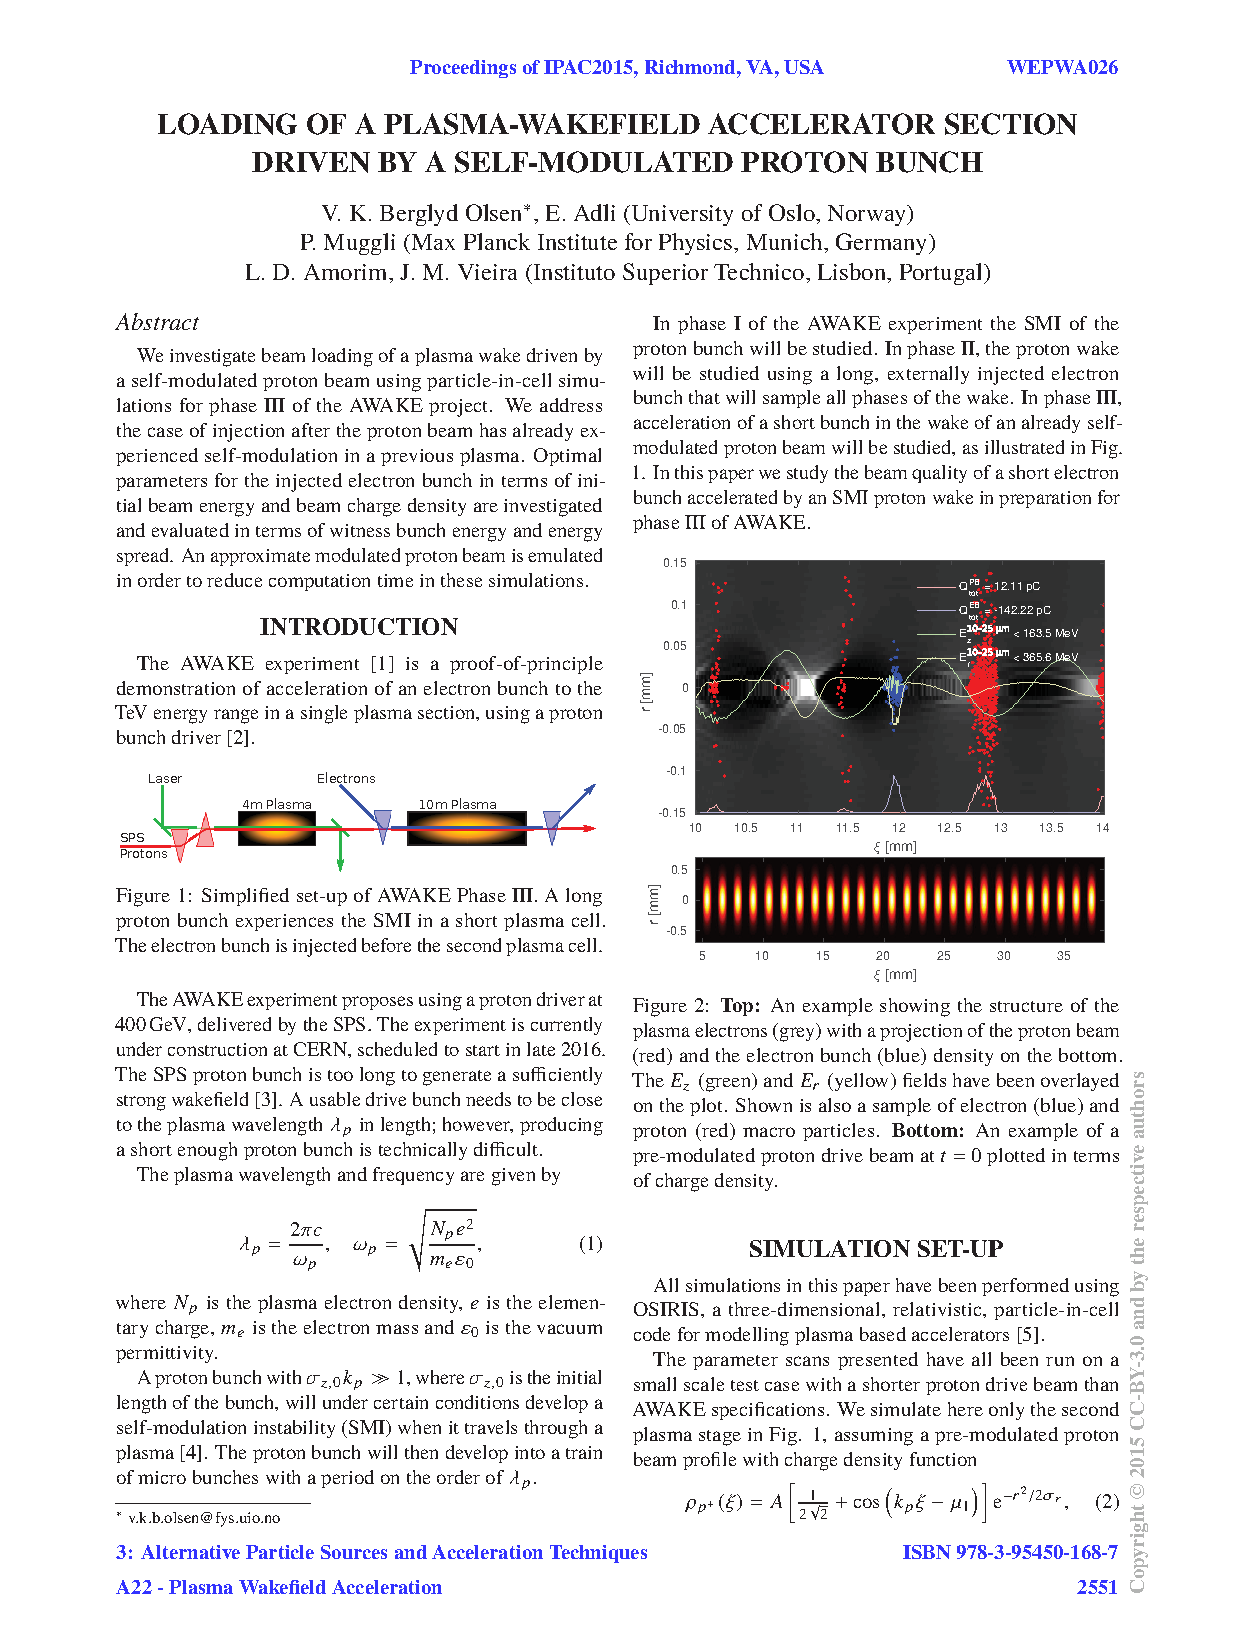
\includepdf[pages=1-last,openright]{Includes/incPaper1.pdf}

\appendix
\backmatter

\end{document}
